\documentclass[aspectratio=169,10pt]{beamer}
\usetheme{Madrid}
\usecolortheme{seahorse}
\usefonttheme{professionalfonts}

\setbeamertemplate{footline}[frame number]
\setbeamertemplate{navigation symbols}{}

\usepackage{amsmath,amssymb,mathtools}
\usepackage{graphicx}
\usepackage{booktabs}
\usepackage{listings}
\usepackage{xcolor}
\usepackage{tikz}
\usetikzlibrary{arrows.meta,positioning}

\graphicspath{{figures/}}

\lstset{
  basicstyle=\ttfamily\scriptsize,
  numbers=left,
  numberstyle=\tiny,
  frame=single,
  backgroundcolor=\color{gray!7},
  commentstyle=\color{green!50!black}\itshape,
  keywordstyle=\color{blue!70!black}\bfseries,
  stringstyle=\color{orange!70!black},
  showstringspaces=false,
  breaklines=true,
  language=Python,
}

\newcommand{\R}{\mathbb{R}}
\newcommand{\E}{\mathbb{E}}
\newcommand{\Pb}{\mathbb{P}}
\newcommand{\Qb}{\mathbb{Q}}
\newcommand{\calK}{\mathcal{K}}
\newcommand{\calF}{\mathcal{F}}
\newcommand{\calP}{\mathcal{P}}
\newcommand{\calS}{\mathcal{S}}
\newcommand{\calA}{\mathcal{A}}
\newcommand{\calT}{\mathcal{T}}
\newcommand{\Theset}{\Theta}
\DeclareMathOperator*{\argmax}{arg\,max}
\DeclareMathOperator{\FCR}{FCR}
\DeclareMathOperator{\FCP}{FCP}
\DeclareMathOperator{\FDR}{FDR}

\title[E-Values -- Ch.13]{Hypothesis Testing with E-Values}
\subtitle{Chapter 13: FCR Control using E-Confidence Intervals}
\author{Based on Ramdas \& Wang}
\date{}

\begin{document}

\begin{frame}
  \titlepage
\end{frame}

\begin{frame}[allowframebreaks]{Outline}
  \tableofcontents
\end{frame}

% ============================================================
\section{Notation you'll need}
% ============================================================

\begin{frame}[allowframebreaks]{Notation you'll need}

  \textbf{Recap: the classical confidence interval (CI).} You already know this from intro stats. Data $X$ is drawn from an unknown distribution $\Pb$, and we want to estimate a functional $\vartheta(\Pb) \in \Theset$ (e.g.\ a mean, a coin's bias, a median). A $(1-\alpha)$-CI is a data-dependent set $C(\alpha) \subseteq \Theset$ such that
  \[
    \Pb\big(\vartheta(\Pb) \in C(\alpha)\big) \geq 1-\alpha \qquad \text{for every } \Pb \text{ under consideration.}
  \]
  This is an \emph{unconditional, pre-registered} guarantee: you must fix which parameter you're covering (and, implicitly, the level $\alpha$) \emph{before} looking at data. That is exactly the assumption we are about to break.

  \framebreak

  \begin{block}{E-confidence interval (e-CI), informally}
    An e-CI is a CI built by \emph{inverting a family of e-values} instead of a family of p-values / test statistics. Concretely, suppose for every candidate value $\theta \in \Theset$ we have an e-variable $E(\theta)$ testing ``$\vartheta(\Pb) = \theta$'' (i.e.\ $\E^{\Pb}[E(\theta)] \leq 1$ whenever $\vartheta(\Pb)=\theta$). Then
    \[
      C(\alpha) := \Big\{ \theta \in \Theset : E(\theta) < \tfrac{1}{\alpha} \Big\}
    \]
    is a $(1-\alpha)$-CI, by Markov's inequality -- and we call it an e-CI. \emph{Every} value of $\alpha$ can be read off from the \emph{same} family of e-values, all at once.
  \end{block}

  \framebreak

  \begin{block}{False coverage rate (FCR) -- the selective-inference problem}
    Suppose you have $K$ parameters $\theta_1^*,\dots,\theta_K^*$ and a $(1-\alpha)$-CI for each. If you look at the data, \emph{select} a data-dependent subset $S \subseteq \{1,\dots,K\}$ of ``interesting'' ones (e.g.\ the largest effects), and only report CIs for $S$, the naive claim ``these are $95\%$ CIs'' is generally \textbf{false}. The false coverage rate is
    \[
      \FCR := \E^{\Pb}\left[ \frac{\sum_{i \in S} \mathbb{1}\{\theta_i^* \notin C_i(\alpha_i)\}}{|S| \vee 1} \right],
    \]
    the \emph{expected} fraction of reported intervals, among the selected ones, that miss their target.
  \end{block}

  \framebreak

  \begin{block}{The selection effect: why FCR $\neq \alpha$}
    Selecting ``the most extreme'' or ``the most significant'' parameters is not innocuous: extremeness in the \emph{estimate} is correlated with the interval being pulled away from the truth (this is the same ``winner's curse'' phenomenon behind regression to the mean). So the CIs you end up reporting are a biased sample of all the CIs you could have reported, and their conditional miscoverage rate can be much higher than the nominal $\alpha$.
  \end{block}

  \framebreak

  \textbf{The FDR analogy (Chapter 9).} This is exactly the CI-analogue of the false discovery rate. Recall: if you test $K$ hypotheses and only report the ones you \emph{reject}, the fraction of those rejections that are false positives (FDP) can badly exceed $\alpha$ unless you correct for the fact that rejection is a data-dependent selection. FDR control (Benjamini--Hochberg, e-BH) fixes this for \emph{point} null hypotheses. FCR control is the same story for \emph{interval estimates}:
  \begin{center}
    \begin{tabular}{ll}
      \toprule
      Chapter 9 (FDR) & Chapter 13 (FCR) \\
      \midrule
      reject/don't-reject $H_i$ & report/don't-report $C_i$ \\
      false positive: $H_i$ true but rejected & false coverage: $\theta_i^* \notin C_i$ but reported \\
      FDP $=$ \# false rejections / \# rejections & FCP $=$ \# false coverages / \# reported \\
      e-BH procedure & e-BY procedure (this chapter) \\
      \bottomrule
    \end{tabular}
  \end{center}
  The tool that makes the e-BY fix work cleanly is precisely the e-CI: because a family of e-CIs is valid \emph{simultaneously at every level $\alpha$}, you're allowed to choose $\alpha_i$ \emph{after} seeing the data (in particular, depending on $|S|$) without breaking validity.

\end{frame}

% ============================================================
\section{13.1 Defining and constructing e-CIs}
% ============================================================

\begin{frame}{13.1 Intuition: why bother with e-CIs at all?}
  A classical $(1-\alpha)$-CI is built for one fixed $\alpha$. If you want a $90\%$ CI \emph{and} a $99\%$ CI, in general you need two separate constructions (or a union bound linking them).

  \vspace{0.3cm}
  An e-CI is built from a family of e-\emph{variables} $\{E(\theta)\}_{\theta \in \Theset}$ testing every possible parameter value. Markov's inequality then gives you a valid CI \emph{at every level $\alpha$ simultaneously}, for free, from that one object:
  \[
    C(\alpha) = \{\theta : E(\theta) < 1/\alpha\}.
  \]
  This ``all levels for the price of one'' property (called \emph{level-free}) is exactly the extra structure that will let us handle a data-dependent selection rule in Section 13.2, and let us merge many uncertainty sets in Section 13.3.
\end{frame}

\begin{frame}[allowframebreaks]{Definition 13.1: families of e-variables and e-CIs}
  Let $\calP$ denote the set of all possible data distributions, $\vartheta:\calP\to\Theset$ a functional of interest, and $\calP_\theta := \{\Pb\in\calP : \vartheta(\Pb)=\theta\}$ the distributions with that functional value.

  \begin{block}{Family of e-variables}
    $\{E(\theta)\}_{\theta\in\Theset}$ is a \emph{family of e-variables} for $\{\calP_\theta\}_{\theta\in\Theset}$ if, for each $\theta$, $E(\theta)$ is an e-variable for $\calP_\theta$, i.e.\ $\E^{\Pb}[E(\theta)] \leq 1$ for every $\Pb \in \calP_\theta$.
  \end{block}

  \begin{block}{$(1-\alpha)$-confidence interval (CI)}
    For fixed $\alpha \in [0,1]$, a set $C(\alpha)\subseteq\Theset$ is a $(1-\alpha)$-CI for $\vartheta$ if $\Pb(\vartheta(\Pb)\in C(\alpha)) \geq 1-\alpha$ for all $\Pb \in \calP$. $\{C(\alpha)\}_{\alpha\in[0,1]}$ is a \emph{family of CIs} if $C(\alpha)$ is a $(1-\alpha)$-CI for every $\alpha$.
  \end{block}

  \framebreak

  \begin{block}{$(1-\alpha)$-e-confidence interval (e-CI)}
    $C(\alpha)$ is a $(1-\alpha)$-e-CI if there \emph{exists} a family of e-variables $\{E(\theta,\alpha)\}_{\theta\in\Theset}$ for $\{\calP_\theta\}_{\theta\in\Theset}$ such that
    \[
      C(\alpha) = \Big\{ \theta \in \Theset : E(\theta,\alpha) < \tfrac{1}{\alpha} \Big\}.
    \]
    $\{C(\alpha)\}_{\alpha\in[0,1]}$ is a \emph{family of e-CIs} if $C(\alpha)$ is an e-CI for every $\alpha$.
  \end{block}

  \begin{block}{Level-free}
    A family of e-CIs is \emph{level-free} if the underlying e-variable $E(\theta,\alpha)$ does \textbf{not} depend on $\alpha$ -- we then write it simply $E(\theta)$, and \emph{one} object $\{E(\theta)\}_{\theta}$ produces valid CIs at \emph{every} level $\alpha$ at once. This is the interesting, powerful case.
  \end{block}

  Convention: $C(0)=\Theset$, $C(1)=\varnothing$, and $C(\alpha)\supseteq C(\alpha')$ for $\alpha\le\alpha'$ (automatic for level-free families).
\end{frame}

\begin{frame}{Two easy facts: e-CI $\Rightarrow$ CI, and CI $\Rightarrow$ e-CI (trivially)}
  \begin{block}{Fact 1: every e-CI is a CI}
    For $\Pb \in \calP_\theta$, Markov's inequality gives
    \[
      \Pb(\theta \notin C(\alpha)) = \Pb\big(E(\theta,\alpha) \geq \tfrac1\alpha\big) \leq \alpha \cdot \E^{\Pb}[E(\theta,\alpha)] \leq \alpha.
    \]
    (This is also why we used strict ``$<1/\alpha$'' rather than ``$\leq$'': it yields the smallest valid e-CI.)
  \end{block}

  \begin{block}{Fact 2: every CI is (trivially) an e-CI}
    Given any $(1-\alpha)$-CI $C(\alpha)$, define the \emph{all-or-nothing} e-variable
    \[
      E(\theta,\alpha) := \frac{1}{\alpha}\, \mathbb{1}\{\theta \notin C(\alpha)\}.
    \]
    Then $\E^{\Pb}[E(\theta,\alpha)] = \tfrac1\alpha \Pb(\theta\notin C(\alpha)) \leq \tfrac1\alpha \cdot \alpha = 1$, so it is a valid e-variable, and one checks $\{\theta : E(\theta,\alpha)<1/\alpha\} = C(\alpha)$ exactly.
  \end{block}
  This embedding is \emph{not} level-free ($E$ depends on $\alpha$ through both the $1/\alpha$ scaling and the set $C(\alpha)$ itself) -- so while every CI ``counts'' as an e-CI, the genuinely useful e-CIs are the level-free ones built from a single underlying e-process, which is what Sections 13.1.1--13.1.2 construct.
\end{frame}

\begin{frame}{Example 13.2: an e-CI for a Gaussian mean, with just $n=1$ observation}
  \begin{block}{A single-observation e-CI}
    For $X_1 \sim N(\mu,\sigma^2)$ with $\sigma^2$ \emph{unknown}, the set
    \[
      X_1 \;\pm\; \alpha^{-1}\exp\!\big((X_1^2-1)/2\big)
    \]
    is a valid $(1-\alpha)$-e-CI for $\mu$, built from the level-free e-variable family $\{|X_1-\mu|\exp((1-X_1^2)/2)\}_{\mu\in\R}$, valid for $\bigcup_{\sigma>0} N(\mu,\sigma^2)$.
  \end{block}
  Here $\alpha$ = miscoverage level, $X_1$ = the single observation, $\mu$ = the candidate mean being tested. In sharp contrast: the classical Student-$t$ CI for $\mu$ needs \emph{at least two} observations to even be well-defined (you need one data point just to estimate the variance). This is a first hint that e-CIs are a genuinely different (not merely repackaged) object -- not just ``inflated classical CIs.''
\end{frame}

\begin{frame}[allowframebreaks]{13.1.1 E-CIs from stopped confidence sequences}
  \textbf{Intuition.} In sequential settings (Chapter 7), data $X_1,X_2,\dots$ arrive one at a time, and we may want a CI that stays valid \emph{no matter when we decide to stop looking} -- even if the stopping time is chosen by peeking at the data. A confidence \emph{sequence} formalizes this.

  \begin{block}{Definition 13.3: confidence sequence}
    Given $\alpha\in[0,1]$, a $(1-\alpha)$-confidence sequence for $\vartheta$ is a sequence of sets $(C^t(\alpha))_{t\in\mathbb{N}}$ such that $C^\tau(\alpha)\subseteq\Theset$ is a $(1-\alpha)$-CI \emph{for any stopping time $\tau$}. Equivalently: $\Pb(\vartheta(\Pb)\in C^t(\alpha) \text{ for all } t\in\mathbb{N}) \geq 1-\alpha$.
  \end{block}
  Here $\tau$ is a random time (possibly data-dependent, e.g.\ ``stop as soon as I'm bored'') satisfying the usual measurability condition $\{\tau\le t\}\in\calF_t$ with respect to the filtration $\{\calF_t\}_{t\geq0}$ generated by the accumulating data.

  \framebreak

  \textbf{Construction.} For fixed $\alpha$, let $E(\theta,\alpha)\equiv\{E_t(\theta,\alpha)\}_{t\geq0}$ be an \emph{e-process} for $\calP_\theta$ (the sequential generalization of an e-value from Chapter 7: at every stopping time, evaluating the process there still gives a valid e-value). Then
  \[
    C^t(\alpha) = \Big\{\theta\in\Theset : E_t(\theta,\alpha) < \tfrac1\alpha\Big\}
  \]
  is a confidence sequence for $\vartheta$, by \emph{Ville's inequality} (the maximal/anytime version of Markov's inequality for nonnegative supermartingales).

  \begin{block}{Proposition 13.4}
    If $\{C^t(\alpha)\}_{t\in\mathbb{N}}$ is constructed as above, then for \emph{any} stopping time $\tau$, $C^\tau(\alpha)$ is an e-CI. Furthermore, if $E(\theta,\alpha)$ does not depend on $\alpha$, then $\{C^\tau(\alpha)\}_{\alpha\in[0,1]}$ is a \emph{level-free} family of e-CIs.
  \end{block}
  This is the key mechanism: because Ville's inequality controls the whole path of the e-process (not just one fixed time), you may stop -- i.e., choose which data-dependent moment to ``read off'' your interval -- \emph{adaptively}, and the guarantee survives.
\end{frame}

\begin{frame}[allowframebreaks]{13.1.2 E-CIs by calibrating CIs}
  \textbf{Intuition.} Suppose you already trust some ordinary (non-e) family of nested CIs $\{C(\alpha)\}_{\alpha}$ (e.g.\ the exact binomial Clopper--Pearson family, or a Wald interval). Can you mechanically convert it into a genuinely \emph{level-free} e-CI family, without redoing any statistics? Yes -- via a \emph{calibrator}.

  \begin{block}{Calibrator (recap)}
    A calibrator $f:[0,1]\to[0,\infty]$ is a nonincreasing function turning any valid p-value $P$ into a valid e-value $f(P)$ (i.e.\ $\E[f(P)]\leq1$ whenever $P$ is a genuine p-value). Its right inverse is $f^{-1}(x) := \sup\{p : f(p)\geq x\}$.
  \end{block}

  \begin{block}{Decreasing / continuous-from-below CI functions}
    Call $C:[0,1]\to2^{\Theset}$ \emph{decreasing} if $\alpha\le\beta \Rightarrow C(\alpha)\supseteq C(\beta)$, and \emph{continuous from below} if $C(\alpha)=\bigcup_{\beta>\alpha}C(\beta)$ for every $\alpha$. (Nested CI families you meet in practice satisfy both.)
  \end{block}

  \framebreak

  \begin{block}{Theorem 13.5: calibrated e-CI}
    If $C$ is decreasing, continuous from below, and $C(\alpha)$ is always a valid $(1-\alpha)$-CI, and $f$ is a calibrator with right inverse $f^{-1}$, then
    \[
      C^{\mathrm{cal}}(\alpha) := C\!\Big(f^{-1}\big(\tfrac1\alpha\big)\Big) \;\supseteq\; C(\alpha)
    \]
    is a $(1-\alpha)$-e-CI, and $\{C^{\mathrm{cal}}(\alpha)\}_{\alpha\in[0,1]}$ is a \emph{level-free} family of e-CIs.
  \end{block}
  \textbf{Proof idea.} Define the ``dual'' p-value $P^{\mathrm{dual}}(\theta):=\inf\{\alpha\in[0,1]:\theta\notin C(\alpha)\}$ -- this is a genuine p-value for $\calP_\theta$ (it is exactly the usual duality between a nested CI family and a p-value function). Then $E^{\mathrm{cal}}(\theta):=f(P^{\mathrm{dual}}(\theta))$ is an e-variable \emph{not depending on $\alpha$} (level-free!), and algebra shows $\{\theta:E^{\mathrm{cal}}(\theta)<1/\alpha\} = C(f^{-1}(1/\alpha))$.

  \framebreak

  \textbf{A concrete calibrator.} The standard family $f_\kappa(p) := \kappa\, p^{\kappa-1}$ for $\kappa\in(0,1)$ satisfies $\int_0^1 f_\kappa(p)\,dp = 1$, so it is a valid calibrator for every $\kappa$. Its inverse is $f_\kappa^{-1}(y) = (\kappa/y)^{1/(1-\kappa)}$, so
  \[
    f_\kappa^{-1}(1/\alpha) = (\kappa\alpha)^{1/(1-\kappa)}.
  \]
  \textbf{Numerically}, for $\alpha=0.05$ and $\kappa=1/2$: $f_\kappa^{-1}(1/\alpha) = (0.5\times0.05)^{2} = 0.000625$. So a calibrated $95\%$ e-CI equals the underlying classical CI at confidence level $1-0.000625 = 99.94\%$ -- i.e.\ \emph{much} wider than the classical $95\%$ CI. \textbf{This is the price of full level-freeness from a generic calibrator}: getting a family valid at \emph{every} $\alpha$ simultaneously, from an arbitrary CI family, is intrinsically conservative. (Optimizing $\kappa$ helps only a little: at $\kappa\approx0.2$ the same computation gives $\approx99.68\%$ instead.) Bespoke constructions -- like Example 13.2, or the e-process/Ville's-inequality route of Section 13.1.1 -- are typically far tighter than this generic recipe.
\end{frame}

\begin{frame}[fragile]{Python: 13.1 -- e-CIs for our running coin example}
  Six coins are each flipped $n=20$ times; unknown to us, every coin is secretly fair ($\theta^*=0.5$). We use \emph{exact} Clopper--Pearson binomial intervals -- which, by the trivial embedding (Fact 2 above), are automatically also e-CIs at each fixed $\alpha$ -- as our running numerical example for the rest of the chapter.
  \begin{lstlisting}
import numpy as np
from scipy.stats import beta as beta_dist

def clopper_pearson(x, n, conf):
    """Exact (1-alpha)-CI for a Binomial(n,theta) proportion."""
    a = 1 - conf
    lo = 0.0 if x == 0 else beta_dist.ppf(a/2, x, n-x+1)
    hi = 1.0 if x == n else beta_dist.ppf(1-a/2, x+1, n-x)
    return lo, hi

coins = {"A": 15, "B": 5, "C": 11, "D": 9, "E": 8, "F": 12}  # heads out of n=20
n, alpha = 20, 0.05
for name, heads in coins.items():
    lo, hi = clopper_pearson(heads, n, 1-alpha)
    phat = heads / n
    print(f"Coin {name}: phat={phat:.2f}  95% e-CI=[{lo:.3f},{hi:.3f}]"
          f"  covers 0.5: {lo <= 0.5 <= hi}")
# Coin A: phat=0.75  95% e-CI=[0.509,0.913]  covers 0.5: False
# Coin B: phat=0.25  95% e-CI=[0.087,0.491]  covers 0.5: False
# Coin C: phat=0.55  95% e-CI=[0.315,0.769]  covers 0.5: True
# Coin D: phat=0.45  95% e-CI=[0.231,0.685]  covers 0.5: True
# Coin E: phat=0.40  95% e-CI=[0.191,0.639]  covers 0.5: True
# Coin F: phat=0.60  95% e-CI=[0.361,0.809]  covers 0.5: True
  \end{lstlisting}
  Already two of the six naive $95\%$ intervals (coins A and B) miss the true bias $0.5$ -- by chance, in this single draw. We will select exactly these two as ``the most extreme,'' and this is where the selection effect strikes.
\end{frame}

% ============================================================
\section{13.2 The e-BY procedure for false coverage rate}
% ============================================================

\begin{frame}{13.2.1 Intuition and setup: the goal of FCR control}
  A scientist observes $\mathbf{X}=(X_1,\dots,X_K)$ and is potentially interested in $K$ functionals $\vartheta_1,\dots,\vartheta_K$, with true values $\theta_i^* := \vartheta_i(\Pb)$. Perhaps they want the $L\geq1$ largest values of $\boldsymbol\theta^*$, or any index exceeding some threshold -- in short, \emph{which} indices matter is often only clear \emph{after} seeing the data.

  \vspace{0.2cm}
  For each $i$, the scientist can build a $(1-\alpha)$-CI $C_i(\alpha)$ from $X_i$. They then pick a data-dependent subset $S=\calS(\mathbf X) \subseteq \calK=\{1,\dots,K\}$ of ``interesting'' parameters, and must choose confidence levels $\{\alpha_i\}_{i\in S}$ (possibly data-dependent too) for the CIs they actually report.

  \begin{block}{False coverage proportion (FCP) and false coverage rate (FCR)}
    \[
      \FCP := \FCP(S,\{\alpha_i\}_{i\in S}) := \frac{\sum_{i\in S}\mathbb{1}\{\theta_i^*\notin C_i(\alpha_i)\}}{|S|\vee 1}, \qquad \FCR := \E^{\Pb}[\FCP].
    \]
    $S$: selected index set; $\alpha_i$: confidence level used for parameter $i$; $|S|\vee1 = \max(|S|,1)$ avoids division by zero. If every $\alpha_i$ equals a common $\gamma$, we write $\FCP(S,\gamma)$.
  \end{block}
  \textbf{Goal:} choose $\{\alpha_i\}_{i\in S}$ so that $\FCR\le\delta$ for a target $\delta$, \emph{for every distribution $\Pb$, and no matter what the selection rule $\calS$ is} -- even if $\calS$ is unknown to us.
\end{frame}

\begin{frame}{The (classical) Benjamini--Yekutieli procedure}
  \textbf{The point of comparison.} The BY procedure's validity depends on assumptions about the dependence in $\mathbf X$ and about $\calS$:
  \begin{itemize}
    \item If $X_1,\dots,X_K$ are \textbf{mutually independent} (and $\calS$ satisfies some regularity conditions), BY sets
    \[
      \alpha_i = \delta\,|S|/K, \qquad i \in S.
    \]
    \item Under \textbf{arbitrary dependence} and an unrestricted/unknown selection rule, BY must instead use the more conservative
    \[
      \alpha_i = \frac{\delta\,|S|}{K\,\ell_K}, \qquad \ell_K := \sum_{i=1}^K \frac1i \approx \log K
    \]
    ($\ell_K$ is the $K$-th harmonic number -- e.g.\ $\ell_6 = 1+\tfrac12+\tfrac13+\tfrac14+\tfrac15+\tfrac16 = 2.45$).
  \end{itemize}
  This is reminiscent of BH vs.\ the log-penalized BH procedure under arbitrary dependence (Chapter 9). The natural hope, by analogy with e-BH (which controls FDR under arbitrary dependence \emph{without} the $\log K$ penalty), is that an \textbf{e-CI-based} procedure can control FCR under arbitrary dependence \emph{without paying the $\ell_K$ tax}. That is exactly the e-BY procedure.
\end{frame}

\begin{frame}{Definition 13.6 and Theorem 13.7: the e-BY procedure}
  \begin{block}{Definition 13.6: e-BY procedure}
    At level $\delta\in[0,1]$, the e-BY procedure sets
    \[
      \alpha_i = \delta\,|S|/K \qquad \text{for each } i \in S.
    \]
  \end{block}
  Same formula as classical BY under independence -- the difference is entirely in \emph{which guarantee it satisfies}, and \emph{why}.

  \begin{block}{Theorem 13.7}
    Let $\{C_i(\alpha)\}_{\alpha\in[0,1]}$ be a \emph{level-free} family of e-CIs, for each $i \in \calK$. Then the e-BY procedure ensures $\FCR \leq \delta$ for any $\delta\in(0,1)$, under \textbf{any} dependence structure between $X_1,\dots,X_K$, and for \textbf{any} selection rule $\calS$ (even unknown to us). In fact, the stronger simultaneous guarantee holds:
    \[
      \E^{\Pb}\Big[\sup_{S\in2^{\calK}}\ \sup_{\delta\in(0,1)}\ \frac{\FCP(S,\delta|S|/K)}{\delta}\Big] \leq 1 \qquad \text{for all } \Pb\in\calP.
    \]
  \end{block}
  \textbf{Why level-free matters:} the proof needs one fixed e-variable $E_i(\theta_i^*)$ per index -- not depending on $\alpha$ -- so that plugging in the data-dependent threshold $\delta|S|/K$ \emph{after} the fact still preserves $\E[E_i(\theta_i^*)]\leq1$.
\end{frame}

\begin{frame}{Proof sketch of Theorem 13.7}
  Write $E_i(\theta_i^*)$ for the level-free e-variable behind $C_i(\cdot)$, so $\theta_i^*\notin C_i(\alpha) \iff E_i(\theta_i^*)\geq1/\alpha$. Then
  \begin{align*}
    \FCR &= \E^{\Pb}\left[\frac{\sum_{i\in S}\mathbb{1}\{\theta_i^*\notin C_i(\delta|S|/K)\}}{|S|\vee1}\right]
    = \E^{\Pb}\left[\frac{\sum_{i\in\calK}\mathbb{1}\{E_i(\theta_i^*)|S|\delta/K>1\}\cdot\mathbb{1}\{i\in S\}}{|S|\vee1}\right]\\
    &\leq \sum_{i\in\calK}\E^{\Pb}\left[\frac{E_i(\theta_i^*)|S|\delta}{K(|S|\vee1)}\right]
    = \sum_{i\in\calK}\frac{\delta}{K}\,\E^{\Pb}\!\left[E_i(\theta_i^*)\cdot\frac{|S|}{|S|\vee1}\right] \leq \sum_{i\in\calK}\frac\delta K = \delta,
  \end{align*}
  using $\mathbb{1}\{x>1\}\le x$ for the first inequality, and $\E[E_i(\theta_i^*)]\le1$ together with $|S|/(|S|\vee1)\le1$ for the second. No independence or knowledge of $\calS$ was used anywhere -- exactly like the ``averaging is always a valid e-merge, regardless of dependence'' fact from Chapter 8. \textbf{Note:} FCR control by e-BY also implies FDR control by e-BH, but not conversely.
\end{frame}

\begin{frame}{Running example, step 1: naive reporting breaks down}
  Recall: $K=6$ coins, $n=20$ flips each, all secretly fair ($\theta_i^*=0.5$); observed heads $15,5,11,9,8,12$ (coins A--F). The scientist's selection rule: report the $L=2$ \emph{most extreme} observed biases -- here, coins A ($\hat p=0.75$) and B ($\hat p=0.25$).

  \begin{center}
    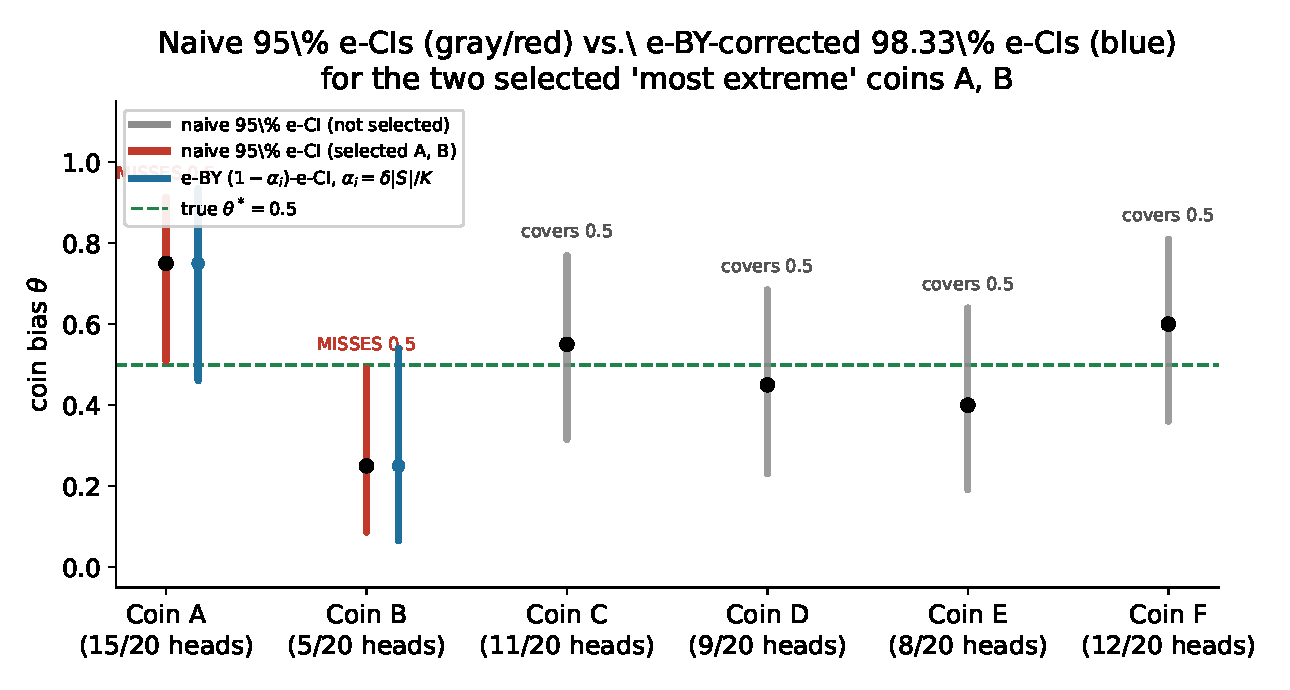
\includegraphics[width=0.85\textwidth]{fig_econfidence_intervals.pdf}
  \end{center}
  If the scientist naively reports ``$95\%$ CIs'' for A and B (i.e.\ uses $\alpha_i=\delta=0.05$, ignoring that they were \emph{selected} for being extreme), \textbf{both} intervals miss the true value $0.5$ in this draw -- not a $5\%$-type event at all for the selected pair.
\end{frame}

\begin{frame}{Running example, step 2: how bad is the naive FCR, really?}
  A single unlucky draw isn't proof of anything -- so we simulate: repeat the ``6 fair coins, flip 20 times, select the 2 most extreme, report nominal $95\%$ CIs'' experiment many times, and track what fraction of the \emph{reported, selected} intervals miss $0.5$.

  \begin{center}
    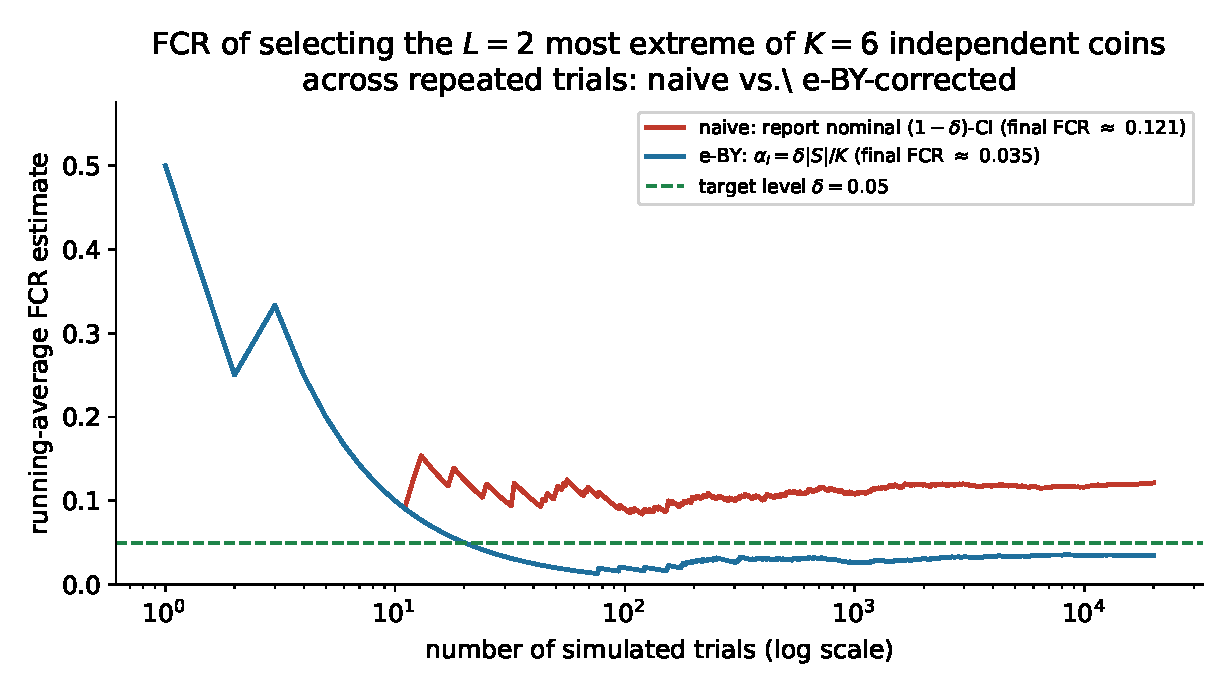
\includegraphics[width=0.8\textwidth]{fig_fcr_simulation.pdf}
  \end{center}
  \textbf{Naive empirical FCR $\approx 0.12$} -- more than double the target $\delta=0.05$. Selecting on extremeness systematically biases the reported intervals away from the truth, exactly as the FDR analogy predicted.
\end{frame}

\begin{frame}{Running example, step 3: applying the e-BY correction}
  \textbf{The fix (Definition 13.6):} since $|S|=2$ and $K=6$, use $\alpha_i = \delta|S|/K = 0.05\times2/6 = 1/60 \approx 0.0167$ for the two selected coins -- i.e., report $(1-\tfrac1{60}) \approx 98.33\%$ intervals instead of $95\%$.

  \begin{block}{Real adjusted numbers}
    \begin{center}
    \begin{tabular}{lccc}
      \toprule
      Coin & naive $95\%$ e-CI & e-BY (98.33\%) e-CI & covers $0.5$? \\
      \midrule
      A ($15/20$) & $[0.509,\ 0.913]$ \ \textcolor{red}{$\times$} & $[0.460,\ 0.934]$ & \textbf{yes} \\
      B ($5/20$)  & $[0.087,\ 0.491]$ \ \textcolor{red}{$\times$} & $[0.066,\ 0.540]$ & \textbf{yes} \\
      \bottomrule
    \end{tabular}
    \end{center}
  \end{block}
  Widening from $95\%$ to $98.33\%$ (a modest correction, since $|S|/K=1/3$ here) is enough to restore coverage in this instance. Over the repeated-trials simulation (previous slide), the \textbf{e-BY-corrected empirical FCR $\approx 0.035 \le \delta = 0.05$}: controlled, as Theorem 13.7 guarantees. And because our coins are independent, this numeric illustration works even with plain (non-e) Clopper--Pearson CIs; the genuine e-BY guarantee (Theorem 13.7) is what lets the \emph{same} formula $\alpha_i=\delta|S|/K$ keep working even if the coins were arbitrarily dependent and $\calS$ were unknown -- unlike classical BY, which would then need the extra $\ell_6=2.45$ penalty, i.e.\ $\alpha_i = 0.05\times2/(6\times2.45) \approx 0.0068$ (a $99.32\%$ interval -- noticeably more conservative).
\end{frame}

\begin{frame}[fragile]{Python: 13.2 -- simulating the FCR of naive vs.\ e-BY reporting}
  \begin{lstlisting}
import numpy as np
from scipy.stats import beta as beta_dist

def clopper_pearson(x, n, conf):
    a = 1 - conf
    lo = 0.0 if x == 0 else beta_dist.ppf(a/2, x, n-x+1)
    hi = 1.0 if x == n else beta_dist.ppf(1-a/2, x+1, n-x)
    return lo, hi

rng = np.random.default_rng(2024)
K, n, L, delta, theta_true = 6, 20, 2, 0.05, 0.5
n_trials = 20000
miss_naive = miss_corrected = 0

for _ in range(n_trials):
    x = rng.binomial(n, theta_true, size=K)              # flip K coins
    phat = x / n
    sel = np.argsort(-np.abs(phat - 0.5))[:L]             # select L most extreme
    alpha_i = delta * L / K                               # e-BY: alpha_i = delta|S|/K
    for i in sel:
        lo_n, hi_n = clopper_pearson(x[i], n, 1 - delta)      # naive: alpha_i = delta
        lo_c, hi_c = clopper_pearson(x[i], n, 1 - alpha_i)    # e-BY corrected
        miss_naive     += not (lo_n <= theta_true <= hi_n)
        miss_corrected += not (lo_c <= theta_true <= hi_c)

print("naive FCR estimate:   ", miss_naive / (n_trials * L))      # ~0.121
print("e-BY corrected FCR:   ", miss_corrected / (n_trials * L))  # ~0.035  (<= 0.05)
  \end{lstlisting}
\end{frame}

% ============================================================
\section{13.3 Combining CIs via majority vote}
% ============================================================

\begin{frame}{13.3 Intuition: many agents, one target, how to merge?}
  Suppose $K$ different ``agents'' each hand you an uncertainty set $C_k$ for the \emph{same} target quantity $c$ -- e.g.\ $K$ different point-estimation methods each with their own CI for a parameter, or $K$ different algorithms each producing a conformal prediction set for the same future outcome. The sets may be built very differently and be arbitrarily dependent (shared data, correlated methods).

  \vspace{0.2cm}
  \textbf{Goal:} combine $C_1,\dots,C_K$, in a black-box manner (only seeing the sets themselves, not how they were built), into one merged set that keeps a valid coverage guarantee while staying reasonably small.

  \begin{block}{Setup (Eq.\ 13.1)}
    Each $C_k = C_k(z)$, $k \in \calK$, based on observed data $z$, satisfies its own marginal guarantee at level $\alpha\in(0,1)$:
    \[
      \Pb(c \in C_k) \geq 1-\alpha, \qquad k \in \calK.
    \]
    Here $c$ is the (possibly random, e.g.\ in conformal prediction) target the agents are all trying to cover.
  \end{block}
\end{frame}

\begin{frame}{Two trivial (bad) solutions: union and intersection}
  \begin{block}{Union $C^J$}
    \[
      C^J := \bigcup_{k=1}^K C_k.
    \]
    Always respects the coverage guarantee (it only grows the set), but is typically \emph{far too large} -- coverage becomes badly inflated (much bigger than $1-\alpha$) at the cost of a useless, oversized set.
  \end{block}
  \begin{block}{Intersection $C^I$}
    \[
      C^I := \bigcap_{k=1}^K C_k.
    \]
    Narrower, but by the union bound only guarantees $\Pb(c\in C^I) \geq 1-K\alpha$ -- \textbf{uninformative} once $K$ is even moderately large (e.g.\ $K\alpha \geq 1$).
  \end{block}
  We want something in between: nearly as small as the individual sets, with a coverage guarantee that doesn't degrade badly with $K$. The answer, again, runs through e-values.
\end{frame}

\begin{frame}{13.3.1 The majority vote procedure}
  \begin{block}{Majority vote set (Eq.\ 13.2)}
    \[
      C^M := \left\{ s \in \calS : \frac1K\sum_{k=1}^K \mathbb{1}\{s\in C_k\} > \frac12 \right\}.
    \]
    $C^M$ contains exactly the points $s$ that \emph{more than half} of the $K$ agents' sets agree contain $c$. ($\calS$ is the space in which the target $c$ lives.)
  \end{block}

  \begin{block}{Theorem 13.8}
    For $K\geq2$ sets satisfying the coverage property above,
    \[
      \Pb(c \in C^M) \geq 1-2\alpha.
    \]
  \end{block}

  \textbf{Proof.} Let $\phi_k := \mathbb{1}\{c\notin C_k\}$, a Bernoulli variable with $\E[\phi_k]\leq\alpha$; then $E_k:=\phi_k/\alpha$ is an e-value, and so is $\bar E:=(E_1+\cdots+E_K)/K$ -- \emph{by the exact same ``averaging is always valid'' fact used throughout this book} (Chapter 8 for merging e-values; the e-BY proof above). Then
  \[
    \Pb(c\notin C^M) = \Pb\Big(\tfrac1K\sum_k\phi_k \geq \tfrac12\Big) = \Pb\big(\bar E \geq \tfrac1{2\alpha}\big) \leq 2\alpha
  \]
  by Markov's inequality. \qed
\end{frame}

\begin{frame}{How tight is $1-2\alpha$, and a general threshold $\tau$}
  The bound $1-2\alpha$ is \emph{worst-case tight}: with $K$ odd and an adversarial joint distribution over the $C_k$'s (either all agents cover $c$, or exactly $\lfloor K/2\rfloor$ do), the miscoverage of majority vote can equal $\alpha K/\lceil K/2\rceil \to 2\alpha$. But it is often much better in practice: if the $C_k$ are \emph{independent}, Hoeffding's inequality gives miscoverage \emph{exponentially small} in $K$ (not just $\le2\alpha$); if the $C_k$ are all identical, coverage is exactly $1-\alpha$.

  \begin{block}{General threshold $\tau$ (Eq.\ 13.4) and Theorem 13.10}
    For any $\tau\in[0,1)$, define
    \[
      C^\tau := \left\{s\in\calS : \frac1K\sum_{k=1}^K\mathbb{1}\{s\in C_k\} > \tau\right\}, \qquad \Pb(c\in C^\tau) \geq 1-\frac{\alpha}{1-\tau}.
    \]
  \end{block}
  Larger $\tau$ $\Rightarrow$ smaller set but weaker guarantee. $\tau=1/2$ recovers majority vote; $\tau=1-1/K$ recovers the intersection $C^I$; $\tau=0$ recovers the union $C^J$ -- one theorem, one dial, interpolating between all our earlier constructions.
\end{frame}

\begin{frame}{Theorem 13.12: majority vote is never more than twice as large}
  \begin{block}{Size bound}
    Let $\nu(\cdot)$ be a measure of size (Lebesgue measure for intervals, counting measure for discrete sets). Then for all $\tau\in[0,1)$,
    \[
      \nu(C^\tau) \leq \frac{1}{K\tau}\sum_{k=1}^K \nu(C_k),
    \]
    and if the input sets are one-dimensional intervals, then for $\tau\in[\tfrac12,1)$, $\nu(C^\tau)\leq\max_k \nu(C_k)$.
  \end{block}
  So at $\tau=1/2$, the merged set's size never exceeds \emph{twice} the average size of the inputs -- and if the inputs are intervals, it never exceeds the size of the single \emph{largest} input interval.

  \vspace{0.2cm}
  \textbf{Numeric caution -- majority vote isn't always the smartest merge.} Take three \emph{nested} intervals $C_1\supset C_2\supset C_3$ of widths $10, 8, 3$. The majority-vote set is $C_2$, width $8$. But simply picking \emph{one} of the three uniformly at random (which still has exact coverage $1-\alpha$!) has expected width $(10+8+3)/3 \approx 7$ -- \emph{smaller} than majority vote. Majority vote's real payoff shows up once we also exploit structure like exchangeability, next.
\end{frame}

\begin{frame}{13.3.2 Improving majority vote: exchangeable sets}
  \textbf{Intuition.} If $C_1,\dots,C_K$ are \emph{exchangeable} (not necessarily independent, but their joint law is permutation-invariant), we can do strictly better than plain majority vote, for free.

  \begin{block}{Sequential majority vote $C^E$ and Theorem 13.13}
    Let $C^M(1{:}k)$ denote the majority vote of just the first $k$ sets. Define
    \[
      C^E := \bigcap_{k=1}^K C^M(1{:}k) = \left\{s\in\calS : \frac1k\sum_{j=1}^k\mathbb{1}\{s\in C_j\}>\tfrac12 \text{ holds for all } k\in\calK\right\}.
    \]
    If $C_1,\dots,C_K$ are exchangeable with coverage $1-\alpha$ each, then $C^E$ has coverage $\geq1-2\alpha$ \emph{and is never worse than plain majority vote}: $C^E \subseteq C^M$.
  \end{block}

  \begin{block}{Corollary 13.14: derandomize by random order}
    If $C_1,\dots,C_K$ are \emph{arbitrarily} dependent, let $\pi$ be an independent uniformly random permutation and apply $C^E$ to the sets in order $\pi(1),\dots,\pi(K)$: this induces exchangeability, so the resulting $C^\pi$ is still a $1-2\alpha$ set, and still $C^\pi\subseteq C^M$.
  \end{block}
  Processing sets in a random order and intersecting the running majority votes can only shrink the merged set, never hurt the guarantee.
\end{frame}

\begin{frame}{Randomized and weighted majority vote}
  \begin{block}{Randomized threshold: $C^R$ (Eq.\ 13.6) and $C^U$ (Eq.\ 13.7)}
    For $U\sim\mathrm{Unif}[0,1]$ independent of the data, with realization $u$:
    \[
      C^R := \Big\{s : \tfrac1K\textstyle\sum_k\mathbb{1}\{s\in C_k\} > \tfrac12+\tfrac u2\Big\}, \qquad
      C^U := \Big\{s : \tfrac1K\textstyle\sum_k\mathbb{1}\{s\in C_k\} > u\Big\}.
    \]
  \end{block}
  \begin{block}{Theorem 13.15}
    $C^R$ has coverage $\geq1-2\alpha$ and is never larger than $C^M$; $C^U$ has coverage $\geq1-\alpha$ (matching the nominal input level!) but is never smaller than $C^R$. The price for $C^U$'s nominal-level coverage is that it needs external randomization.
  \end{block}

  \begin{block}{Weighted vote $C^W$ (Eq.\ 13.8) and Theorem 13.16}
    With prior weights $w_k\in[0,1]$, $\sum_k w_k=1$ (fixed \emph{before} seeing the sets, e.g.\ reflecting trust in agent $k$):
    \[
      C^W := \Big\{s : \textstyle\sum_k w_k\,\mathbb{1}\{s\in C_k\} > \tfrac12+\tfrac u2\Big\}, \qquad
      \Pb(c\in C^W)\geq1-2\alpha, \quad \nu(C^W)\leq 2\textstyle\sum_k w_k\,\nu(C_k).
    \]
  \end{block}
  Equal weights $w_k=1/K$ recovers $C^R$. Proposition 13.17 further allows each agent to have its \emph{own} level $\alpha_k$: $\Pb(c\in C^W)\geq1-2\sum_k w_k\alpha_k$.
\end{frame}

\begin{frame}{Majority vote for confidence sequences and derandomizing estimators}
  \begin{block}{Proposition 13.18 and Theorem 13.19}
    $K$ different $(1-\alpha)$ confidence \emph{sequences} tracked in parallel: their majority vote is a $(1-2\alpha)$ confidence sequence. If the sequences arrive one-at-a-time (exchangeably, or in random order), the \emph{running} majority vote $C^E(1{:}t) := \bigcap_{i=1}^t C^M(1{:}i)$ satisfies
    \[
      \Pb\big(\exists\, t\geq1 : c\notin C^E(1{:}t)\big) \leq 2\alpha.
    \]
  \end{block}
  This lets you \emph{derandomize on the fly}: keep merging estimators/CIs as they arrive, watch the sequence stabilize, and stop whenever you like -- the guarantee holds for whatever (random, data-dependent) stopping point you chose.

  \begin{block}{Corollary 13.21: derandomizing point estimators}
    If $\hat\theta_1,\dots,\hat\theta_K$ are estimators with $\Pb(|\hat\theta_k-\theta|\le w(n,\alpha))\geq1-\alpha$, their \emph{median} $\hat\theta_{(\lceil K/2\rceil)}$ satisfies $\Pb(|\hat\theta_{(\lceil K/2\rceil)}-\theta|\le w(n,\alpha))\geq1-2\alpha$ -- and this holds simultaneously over all $K$ if the estimators are exchangeable.
  \end{block}
\end{frame}

\begin{frame}{13.3.3 Median of midpoints, and derandomizing median-of-means}
  \begin{block}{Theorem 13.20: median of midpoints}
    If $C_1,\dots,C_K$ are intervals of the \emph{same width} with midpoints $c_1,\dots,c_K$, then the majority vote $C^M$ is contained in (and hence no wider than) the interval centered at the \emph{median} midpoint $c_{(\lceil K/2\rceil)}$ -- a much cheaper computation than the general majority-vote construction, exactly recovering $C^M$ when $\bigcap_k C_k\ne\varnothing$.
  \end{block}

  \begin{block}{Corollaries 13.21--13.22: median-of-median-of-means (MoMoM)}
    The median-of-means (MoM) estimator $\hat\mu^{\mathrm{MoM}}$ (splitting $n$ points into $B$ buckets, averaging within each, then taking the median across buckets) gives sub-Gaussian tails but is \emph{randomized} by the random bucketing. Repeating MoM independently $K$ times and taking the \emph{median of the $K$ resulting estimates} (``MoMoM'') derandomizes it, at the mild cost of doubling the deviation probability: $\Pb(\exists K\geq1: |\hat\mu_K^{\mathrm{MoMoM}}-\mu|\geq C\sigma\sqrt{t/n}) \leq 4e^{-t}$ (vs.\ $2e^{-t}$ for one run of MoM) -- while the simultaneity over $K$ means you can watch the estimate stabilize and stop adaptively.
  \end{block}
\end{frame}

\begin{frame}{13.3.4 Empirical examples from the book}
  \textbf{Lasso conformal prediction.} $K=20$ conformal prediction intervals (one per tuning parameter $\lambda$) merged with equal weights $w_k=1/K$ at $\alpha=0.05$: empirical coverage of $C^M$ was $0.97$, of the smaller $C^R$ was $0.92$ -- both comfortably above the guaranteed $1-2\alpha=0.90$, and the randomized-permutation version $C^\pi$ achieved $0.93$ coverage with smaller sets than plain majority vote.

  \begin{block}{Parkinson's UPDRS prediction (real data, $K=4$ algorithms)}
    \begin{center}
    \begin{tabular}{lcccccccc}
      \toprule
      & LM & Lasso & RF & NN & $C^M$ & $C^R$ & $C^U$ & $C^\pi$ \\
      \midrule
      Coverage & 0.958 & 0.960 & 0.949 & 0.961 & 0.951 & 0.923 & 0.961 & 0.918 \\
      Width & 40.1 & 40.2 & 13.3 & 32.5 & 29.5 & 20.6 & 32.5 & 20.7 \\
      \bottomrule
    \end{tabular}
    \end{center}
  \end{block}
  All merges achieve good coverage; $C^R$ and $C^\pi$ are markedly narrower than the raw linear-model / lasso / neural-net intervals, at only a modest coverage cost relative to the (already excellent) random forest. Since random forest performs best individually here, upweighting it in $C^W$ would shrink the merged set further.
\end{frame}

\begin{frame}[fragile]{Python: 13.3 -- majority vote on a small numeric example}
  \begin{lstlisting}
import numpy as np

# 5 arbitrarily-dependent intervals for the same target c, each with
# marginal coverage >= 1-alpha (alpha = 0.10 here, so 1-2*alpha = 0.80 guaranteed)
C = [(1.0, 6.5), (2.0, 6.0), (2.3, 5.0), (2.6, 7.0), (3.4, 4.6)]   # (lo, hi)
K = len(C)

def majority_vote(intervals, tau=0.5, n_grid=200000, lo_grid=0.0, hi_grid=8.0):
    """Approximate C^tau by evaluating the vote fraction on a fine grid."""
    s = np.linspace(lo_grid, hi_grid, n_grid)
    votes = np.zeros_like(s)
    for lo, hi in intervals:
        votes += (s >= lo) & (s <= hi)
    in_set = (votes / K) > tau
    if not in_set.any():
        return None
    pts = s[in_set]
    return float(pts.min()), float(pts.max())

print("Majority vote C^M (tau=1/2):", majority_vote(C, tau=0.5))
# -> approx (2.3, 6.0): the region at least 3 of the 5 intervals agree on

# Median-of-midpoints shortcut (Theorem 13.20), valid since here all
# intervals happen to have the same width after recentering by hand:
widths = [hi - lo for lo, hi in C]
print("interval widths:", widths)         # not all equal in general;
                                           # the shortcut needs equal widths
  \end{lstlisting}
\end{frame}

% ============================================================
\section{Take-aways}
% ============================================================

\begin{frame}[allowframebreaks]{Chapter 13 summary}
  \begin{itemize}
    \item An \textbf{e-CI} is a confidence set built by inverting a family of e-variables, $C(\alpha)=\{\theta : E(\theta,\alpha)<1/\alpha\}$; when the underlying e-variable doesn't depend on $\alpha$ (\emph{level-free}), one object gives valid CIs at \emph{every} level simultaneously. Every CI is trivially an e-CI, and every e-CI is a genuine CI (Markov's inequality).
    \item Level-free e-CIs can be built from stopped confidence sequences / e-processes (Ville's inequality; Section 13.1.1), or by \emph{calibrating} an existing nested CI family with a calibrator (Theorem 13.5; Section 13.1.2) -- though generic calibration is noticeably conservative.
    \item \textbf{FCR} is the CI-analogue of FDR (Chapter 9): reporting CIs only for a data-dependently \emph{selected} subset of parameters can badly break the nominal coverage, exactly as reporting only ``significant'' tests breaks FWER/type-I control.
    \item The \textbf{e-BY procedure} (Definition 13.6) sets $\alpha_i=\delta|S|/K$ for the selected indices; using level-free e-CIs, Theorem 13.7 guarantees $\FCR\le\delta$ under \emph{arbitrary} dependence and an \emph{arbitrary/unknown} selection rule -- unlike classical BY, which needs independence (or an extra $\log K$-type penalty $\ell_K$) for the analogous guarantee.
    \item Our running numeric example: $6$ coins, naive $95\%$ CIs for the $2$ ``most extreme'' miss the truth in simulation about $12\%$ of the time; the e-BY correction ($\alpha_i=1/60$, i.e.\ $98.33\%$ CIs) brings this down to about $3.5\%$, safely below the $\delta=0.05$ target.
    \item \textbf{Majority vote} merges $K$ arbitrarily-dependent uncertainty sets for a shared target into one set with coverage $\geq1-2\alpha$, using at most twice the average size of the inputs -- with exchangeable, randomized, and weighted variants that only ever shrink the merged set while preserving the guarantee.
  \end{itemize}
\end{frame}

\end{document}
